\documentclass{beamer}
\usepackage{amssymb,amsmath,amsfonts,pdfpages,color, url}
\usepackage{booktabs}
\usepackage{wrapfig}
\usepackage{amsmath}
\usepackage{multirow}

\setbeamertemplate{navigation symbols}{}
\usetheme{Montpellier}

\setbeamertemplate{footline}[page number]


\def\dis{\mathop{\displaystyle}}
\def\argmin{\mathop{\rm argmin}}


\newcommand{\E}{\mathbb{E}}
\newcommand{\jeff}[1]{{\color{blue}$\langle$Jeff: #1$\rangle$}}
\newcommand{\dgen}{\ensuremath{\mathtt{d}}}



\title{Efficient Trajectory Retrieval}
\author{By Hasan Pourmahmood}
\date{December 6, 2021}

\begin{document}

\frame{\titlepage}


\section{Motivation}

\begin{frame} 
\frametitle{Trajectory}
\begin{block}{}
A spatial trajectory (also called a piece-wise linear curve) is a sequence of waypoints along with a time stamp, i.e. 
$$T=\{(x_1, y_1, t_1), \ldots, (x_n, y_n, t_n)\}.$$
\begin{figure}[h] 
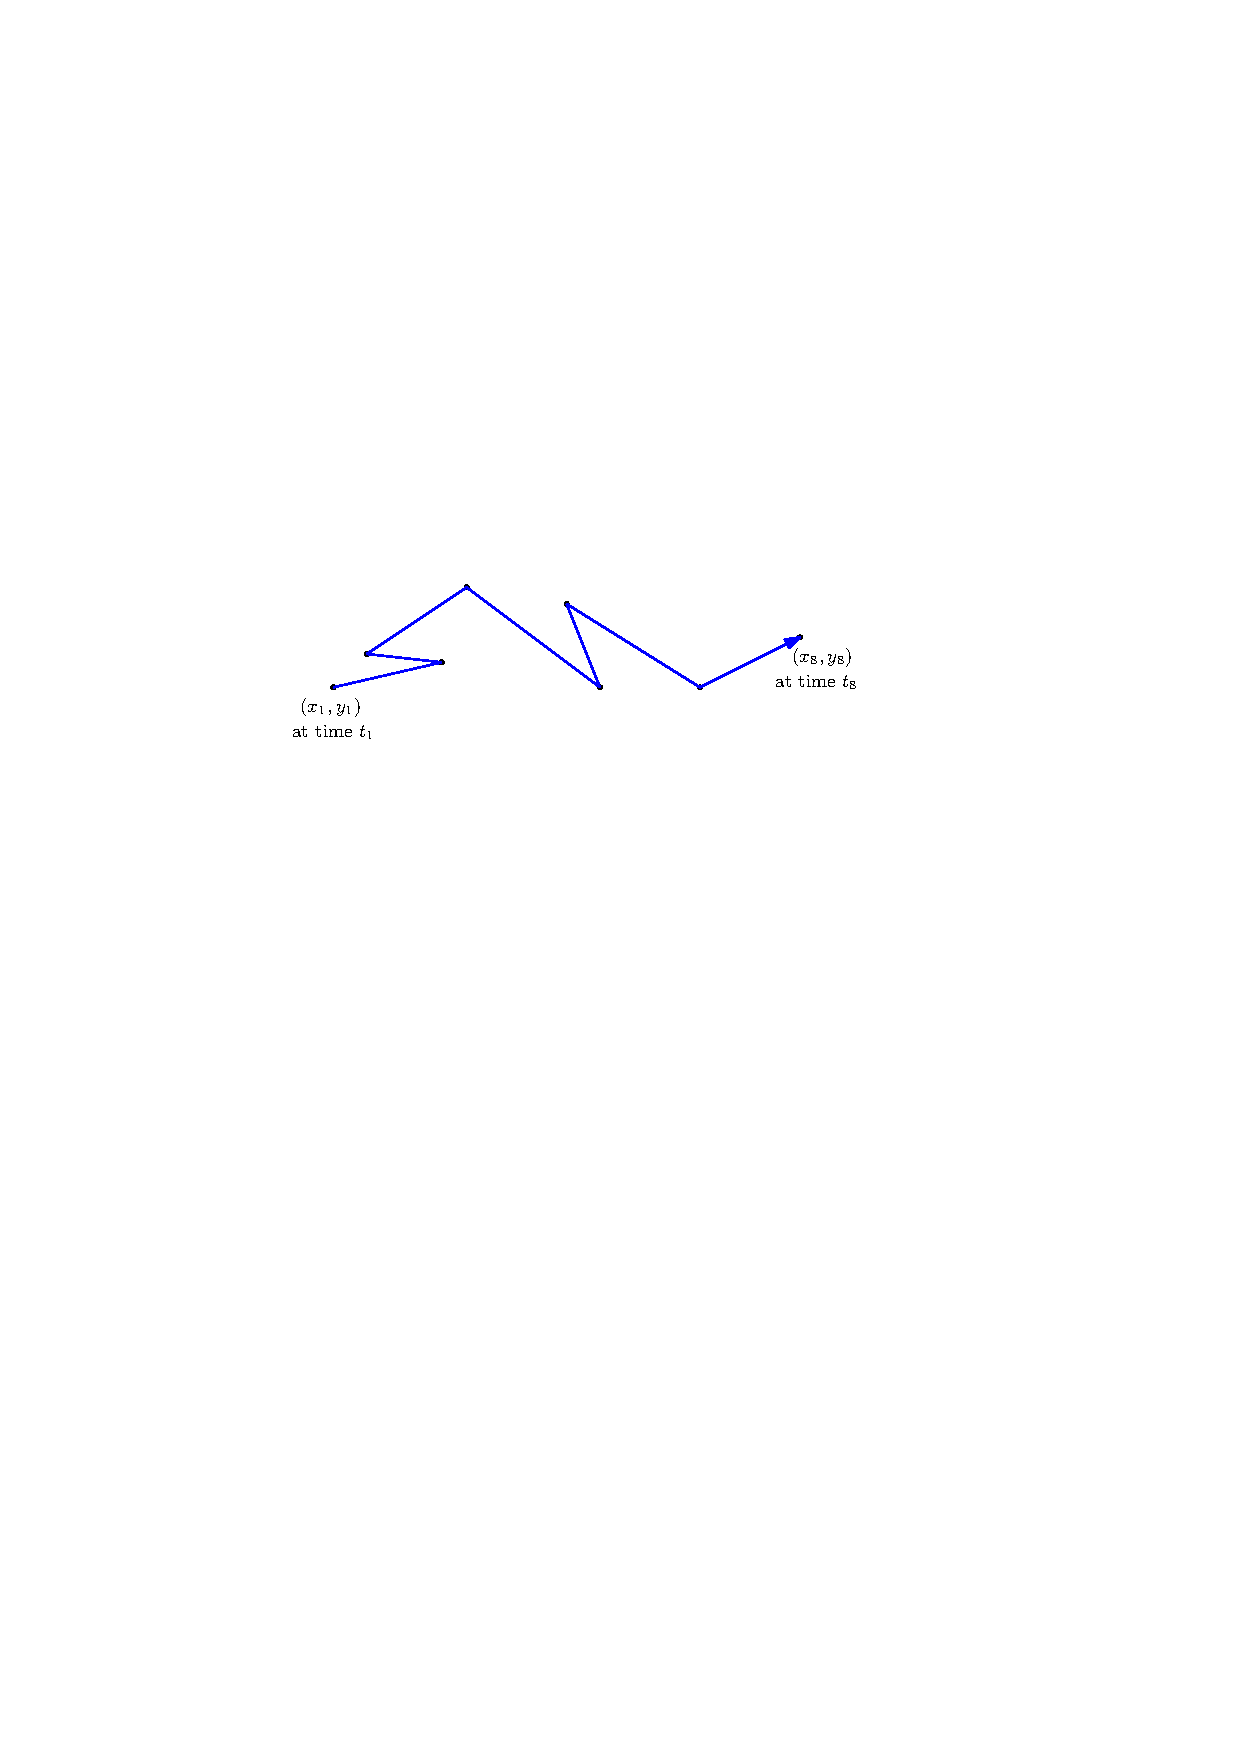
\includegraphics[width=0.8 \textwidth]{trajectory} 
\end{figure}  \vspace{-1mm}
\end{block} 
\end{frame}




\begin{frame}
\frametitle{}
\begin{block}{Popular Distances}
\begin{itemize}
\item [$\blacktriangleright$] Dynamic Time Warping distance (DTW)

\item [$\blacktriangleright$] Fr\'echet distance 

\item [$\blacktriangleright$] Discrete Fr\'echet distance \pause 
\end{itemize}
Complexity: {\color{orange} Quadratic in number of waypoints $O(mn)$}.
\end{block} \pause

\begin{block}{Queryies}
\begin{itemize}
\item {\color{blue} $k$-NN queries:} find $k$ nearest trajectories from data to the given query trajectory $Q$.
\item {\color{blue} Range queries:} find all trajectories within distance $r$ from data to the given query trajectory $Q$.
\end{itemize}
\end{block} \pause

\begin{block}{Applications}
{\small Route extraction, route recommendation, ML on trajectory datasets, ...}
\end{block}
\end{frame}




\section{Information Retrieval}

\begin{frame}
\frametitle{Vector space model using grid structure}  \vspace{-9mm}
\begin{block}{} 
\begin{figure}[h] 
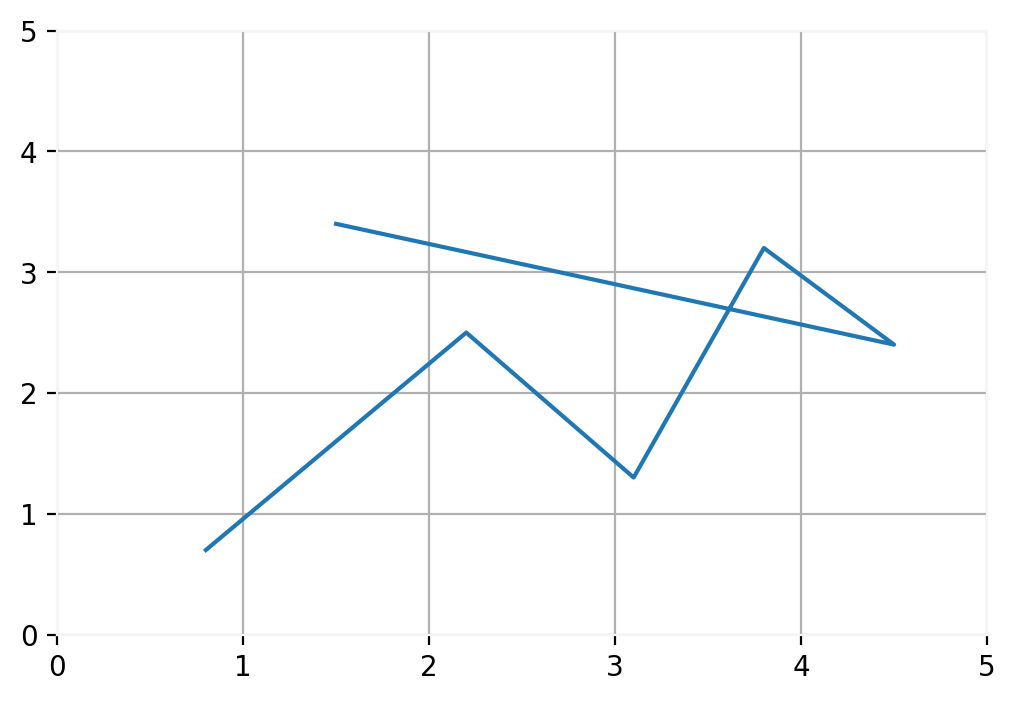
\includegraphics[width=0.6 \textwidth]{grid} 
\end{figure}  \vspace{-3mm} \pause

\begin{itemize}
\item {\bf Vocabulary:} the whole set of grids $\{c_1, \ldots, c_n\}$
\item {\bf Document:} trajectory
\item {\bf Term:} a grid
\end{itemize}
\end{block}
\end{frame}



\begin{frame}
\frametitle{Vector space model using grid structure}  \vspace{-9mm}
\begin{block}{} 
\begin{figure}[h] 
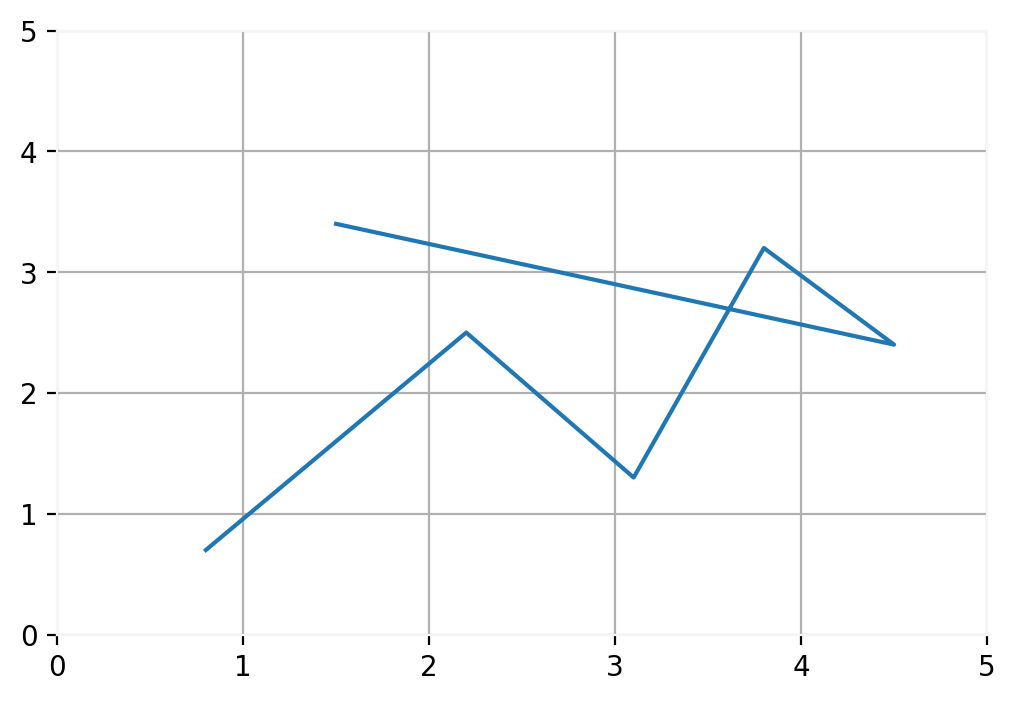
\includegraphics[width=0.6 \textwidth]{grid} 
\end{figure}  \vspace{-4mm} 

{\color{blue} Binary representation:} 

$\tilde{T} = [1,1,0,0,0,0,1,1,1,0,0,1,1,1,1,0,1,1,1,0,0,0,0,0,0]$  \vspace{1mm} \pause

{\color{blue} Frequency representation:} 

$\tilde{T}= [1,1,0,0,0,0,1,1,1,0,0,1, \underbrace{2, 2}_{\color{magenta} 13, 14},1,0,1,1,1,0,0,0,0,0,0]$
\end{block}
\end{frame}


\begin{frame}
\frametitle{Grid aggregate distance (GAD)} 
\begin{block}{} 
Consider a cell similarity matrix $C_{n \times n} = (sim(c_i, c_j))_{i,j=1}^n$ ($c_i$ is the center of cell $i$), like 
\[
{\color{orange} sim(c_i, c_j) = e^{-\|c_i-c_j\|^2/\sigma^2}} \pause
\] 
which is applied in experiments. Then
\[
{\color{orange} GAD(T_1, T_2) = \sqrt{(\tilde{T}_1 - \tilde{T}_2)^t \cdot C \cdot (\tilde{T}_1 - \tilde{T}_2)}} \pause
\] 

{\color{magenta} Problem:} The number of grids $n$ is high (in experiments it is set to 2500), and so operations would be inefficient. \vspace{3mm} \pause

{\color{magenta} We should address this problem. How?}
\end{block}
\end{frame}



\begin{frame}
\begin{block}{} 
\frametitle{Dimensionality reduction technique}  

\begin{itemize}
\item Decompose $C$ to $C = P \Delta P^t$, \pause
\item $\tilde{\tilde{D}} = \Delta^{1/2} P^t \tilde{D}$, where $\tilde{D}$ is the binary/frequency-type representation of data $D$, \pause
\item Use {\color{orange} SVD} for $\tilde{\tilde{D}} $ to reduce the dimension (in experiments 2500 is reduced to 25 and 100), \pause
\item Employ {\color{orange} Euclidean distance} for new short vectors as an approximation for GAD between trajectories, \pause
\item When a query comes, do the same and consult the index to retrieve appropriate trajectories.
\end{itemize}
\end{block}
\end{frame}




\section{Experiments and Evaluation}

\begin{frame}
\frametitle{Data Sets} 
\begin{block}{} \vspace{-8mm}
\begin{table}[!htbp]
{\footnotesize
\centering
\begin{tabular}{rccccc}
 	{\bf Data } 	&  	{\bf Size}  	& 	{\bf Cleaned}  	& {\bf Sample}	& {\bf Grids}	&	{\bf Reduced dim}	\\ \midrule
 	Car-Bus   		& 	163   	& 	105 			&	105		&	2500		&	25	\\ \midrule
	Characters   	& 	2858	    	& 	2858 		&	300		&	2500		&	25	\\ \midrule
 	Geolife  		&   	17621  	&      14187		&	1000		&	2500		&	100	\\ \bottomrule 
\end{tabular} 
\caption{\footnotesize Overview of data sets}
\label{table: datasets} 
}
\end{table} \vspace{-6mm} \pause

\begin{figure}[h] 
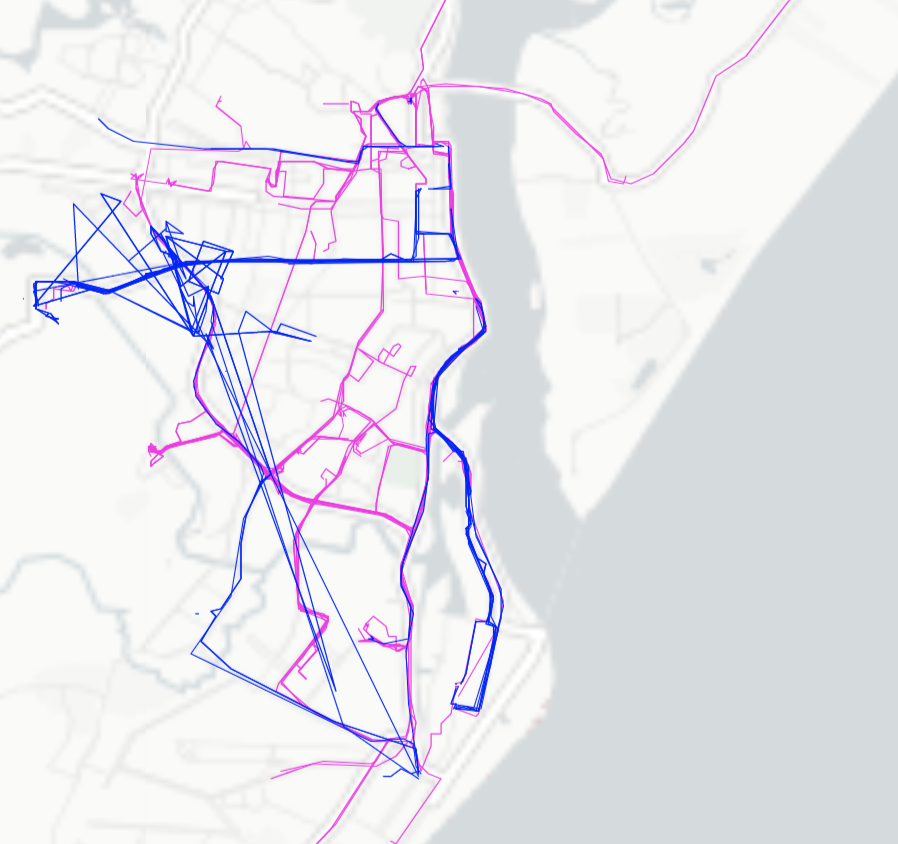
\includegraphics[width=0.28 \textwidth]{car-bus} 
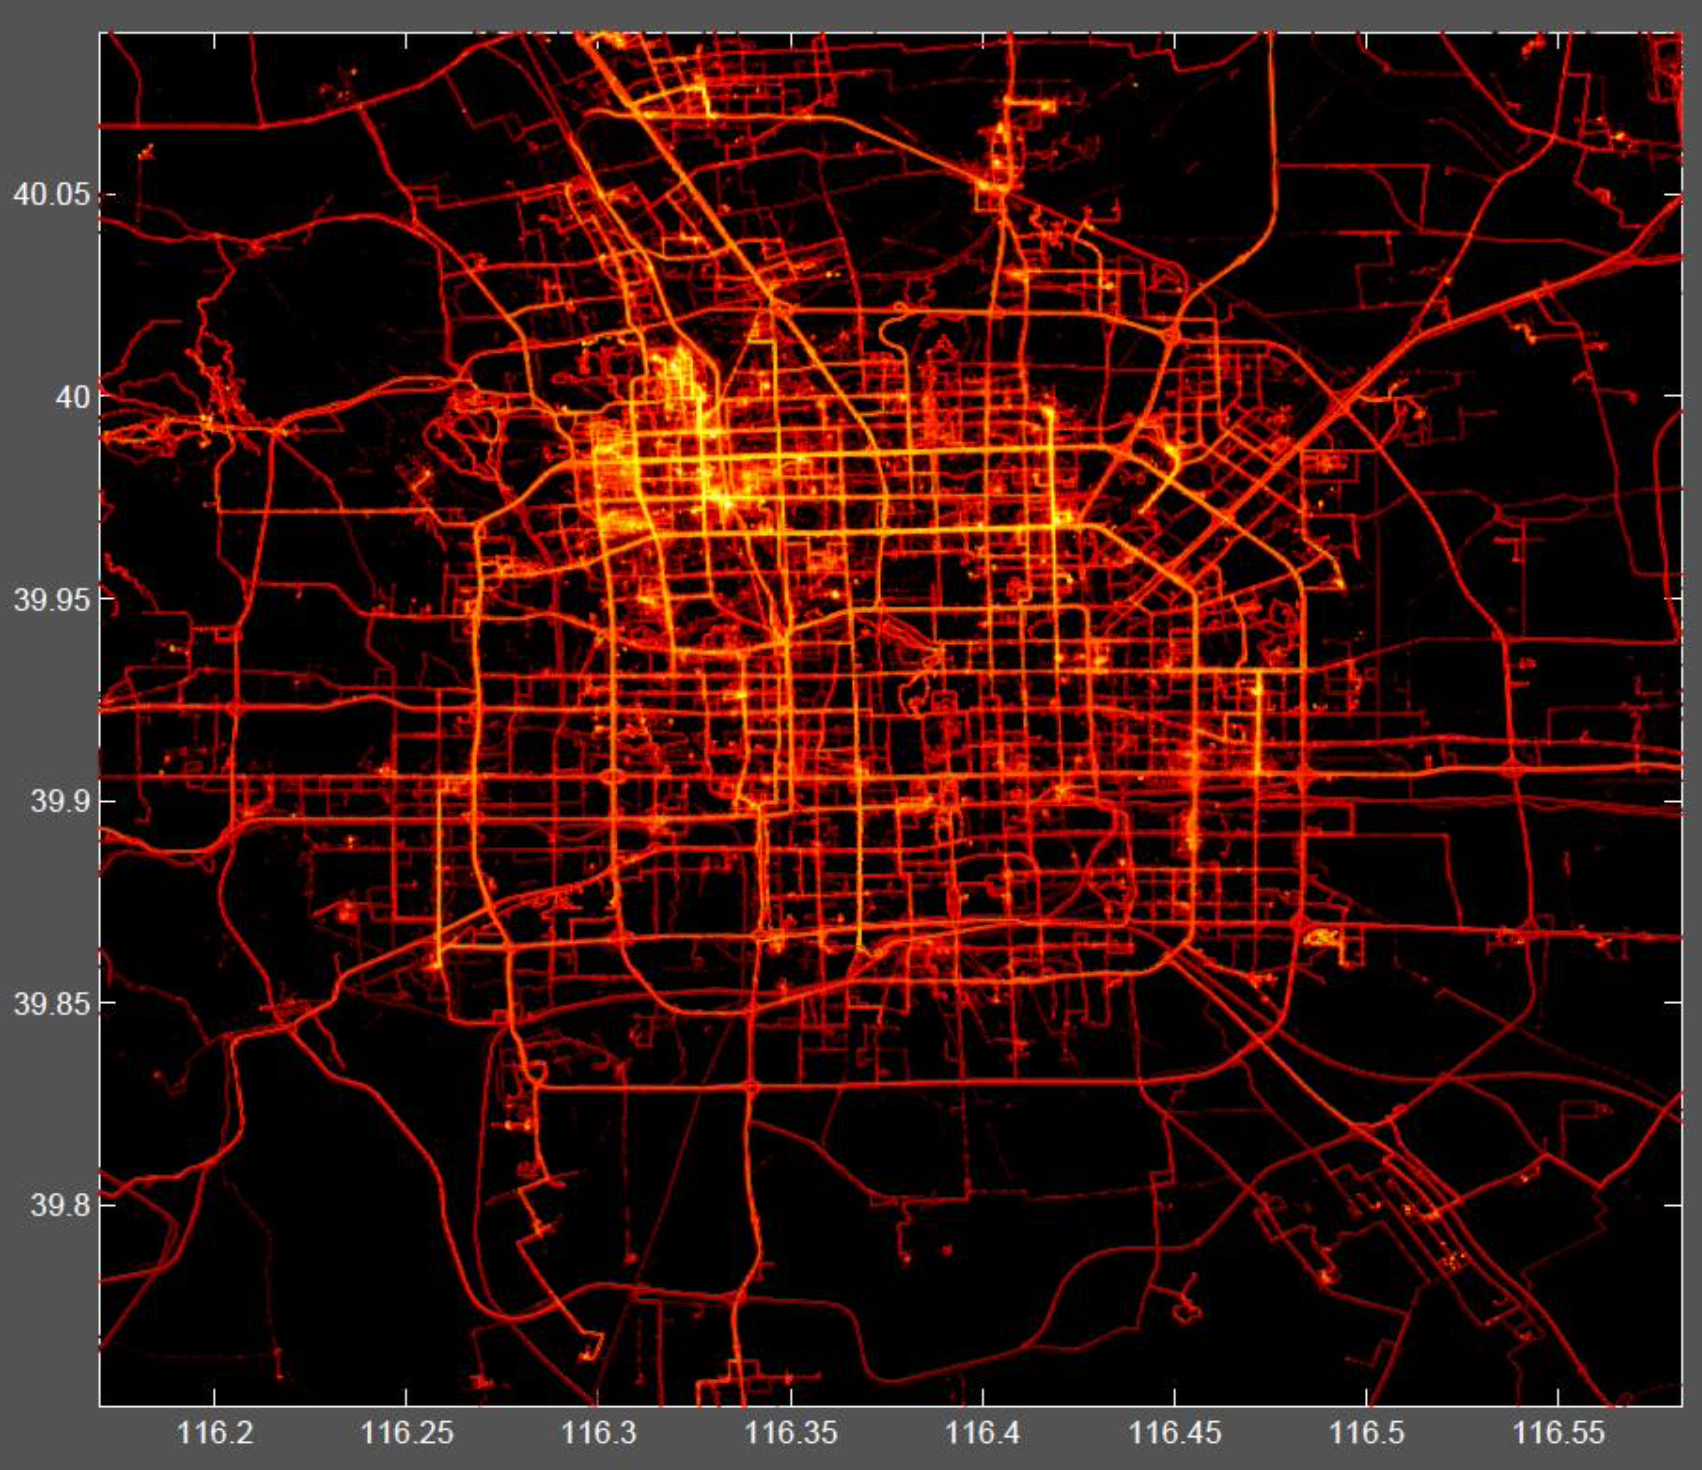
\includegraphics[width=0.3 \textwidth]{Geolife}
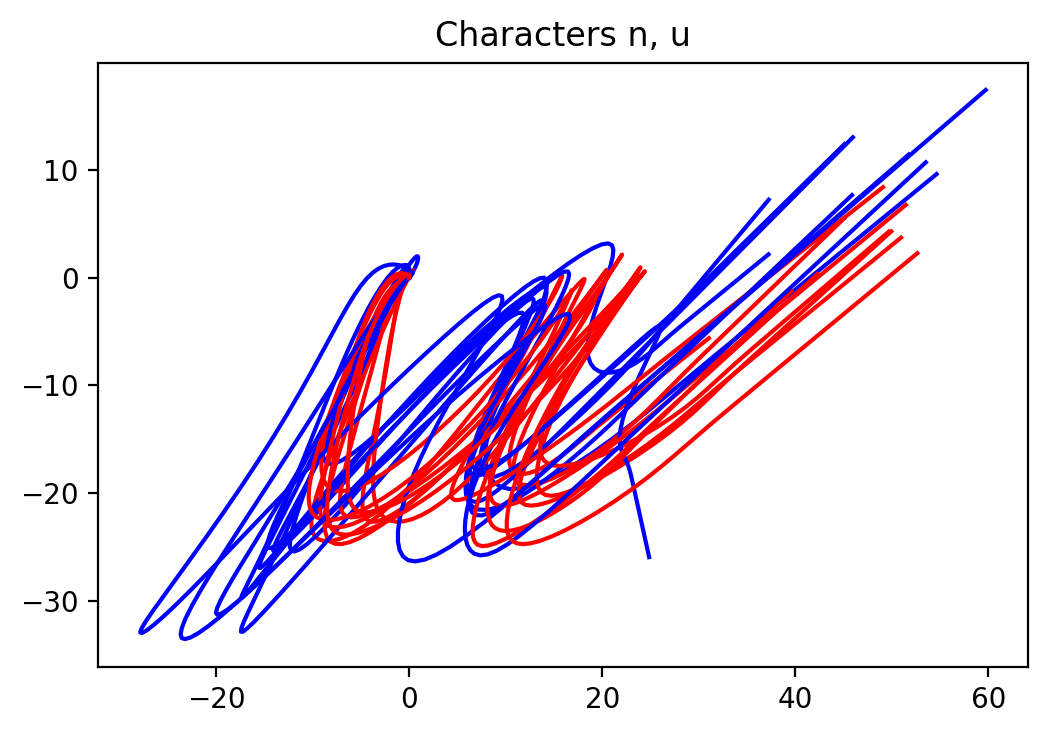
\includegraphics[width=0.35 \textwidth]{Characters-2-fig}
\caption{Car-Bus (left), Geolife (middle), Characters: letters n, u (right).}
\label{characters}
\end{figure}
\end{block}
\end{frame}




\subsection{Car-Bus}

\begin{frame}
\frametitle{kNN Queries (Car-Bus)} 
\begin{block}{} \vspace{-3mm}
\begin{table}[!htbp]
{\footnotesize
\centering
\begin{tabular}{rcccc}
 	{\bf k } 	& {\bf Precision/Recall}	&	{\bf MAP}	 & {\bf nDCG@5}	& {\bf nDCG@10} \\ \midrule
 	5   		& 		0.8781   	 	&	0.8929	 & 0.9400			& 0.9646	\\ \midrule
	10   		& 		0.9143    	 	&	0.8996	 & 0.7902			& 0.9588	\\ \midrule
 	20  		&   		0.9576   		&	0.9240	 & 0.5907  		& 0.8210	\\ \bottomrule 
\end{tabular} 
\caption{\footnotesize Performance with binary representation} \vspace{3mm}

\centering
\begin{tabular}{rcccc}
 	{\bf k } 	& {\bf Precision/Recall}	&	{\bf MAP}	 & {\bf nDCG@5}	& {\bf nDCG@10} \\ \midrule
 	5   		& 	0.9314   		 	&	0.9579	& 0.9809			& 0.9942	\\ \midrule
	10   		& 	0.9343    		 	&	0.9496	& 0.8210			& 0.9856	\\ \midrule
 	20  		&   	0.9700   			&	0.9530	& 0.6024  			& 0.8298	\\ \bottomrule 
\end{tabular} 
\caption{\footnotesize Performance with frequency representation}
\label{table: car-bus binary} 
}
\end{table}
\end{block}
\end{frame}



\begin{frame}
\frametitle{Range Queries (Car-Bus)} 
\begin{block}{} \vspace{-3mm}
\begin{table}[!htbp]
{\footnotesize
\centering
\begin{tabular}{rccccc}
 	{\bf r } 	& {\bf Precision}& {\bf Recall}	&	{\bf MAP}	 & {\bf nDCG@5}	& {\bf nDCG@10} \\ \midrule
 	0.002   	& 	0.8634    	& 	0.9657 	&	0.8061	 & 0.7491			& 0.6313	\\ \midrule
	0.005   	& 	0.8775    	& 	0.9162 	&	0.7228	 & 0.8955			& 0.8895	\\ \midrule
 	0.01 		&   	0.9171   	&      0.9171	&	0.7274	 & 0.9400  		& 0.9588	\\ \bottomrule
\end{tabular} 
\caption{\footnotesize Performance with binary representation} \vspace{3mm}

\centering
\begin{tabular}{rccccc}
 	{\bf r } 	& {\bf Precision}& {\bf Recall}	&	{\bf MAP}	 & {\bf nDCG@5}	& {\bf nDCG@10} \\ \midrule
 	0.002   	& 	0.9914    	& 	1 		&	0.9914	 & 0.5175			& 0.3599	\\ \midrule
	0.005  	& 	0.9603    	& 	1 		&	0.9603	 & 0.5393			& 0.3792	\\ \midrule
 	0.01 		&   	0.9056   	&      0.9990	&	0.8914	 & 0.6260  		& 0.4737	\\ \bottomrule
\end{tabular} 
\caption{\footnotesize Performance with frequency representation}
\label{table: car-bus multipass} 
}
\end{table}
\end{block}
\end{frame}


\begin{frame}
\frametitle{Precision} 
\begin{block}{} \vspace{-1cm}
\begin{figure}[h] 
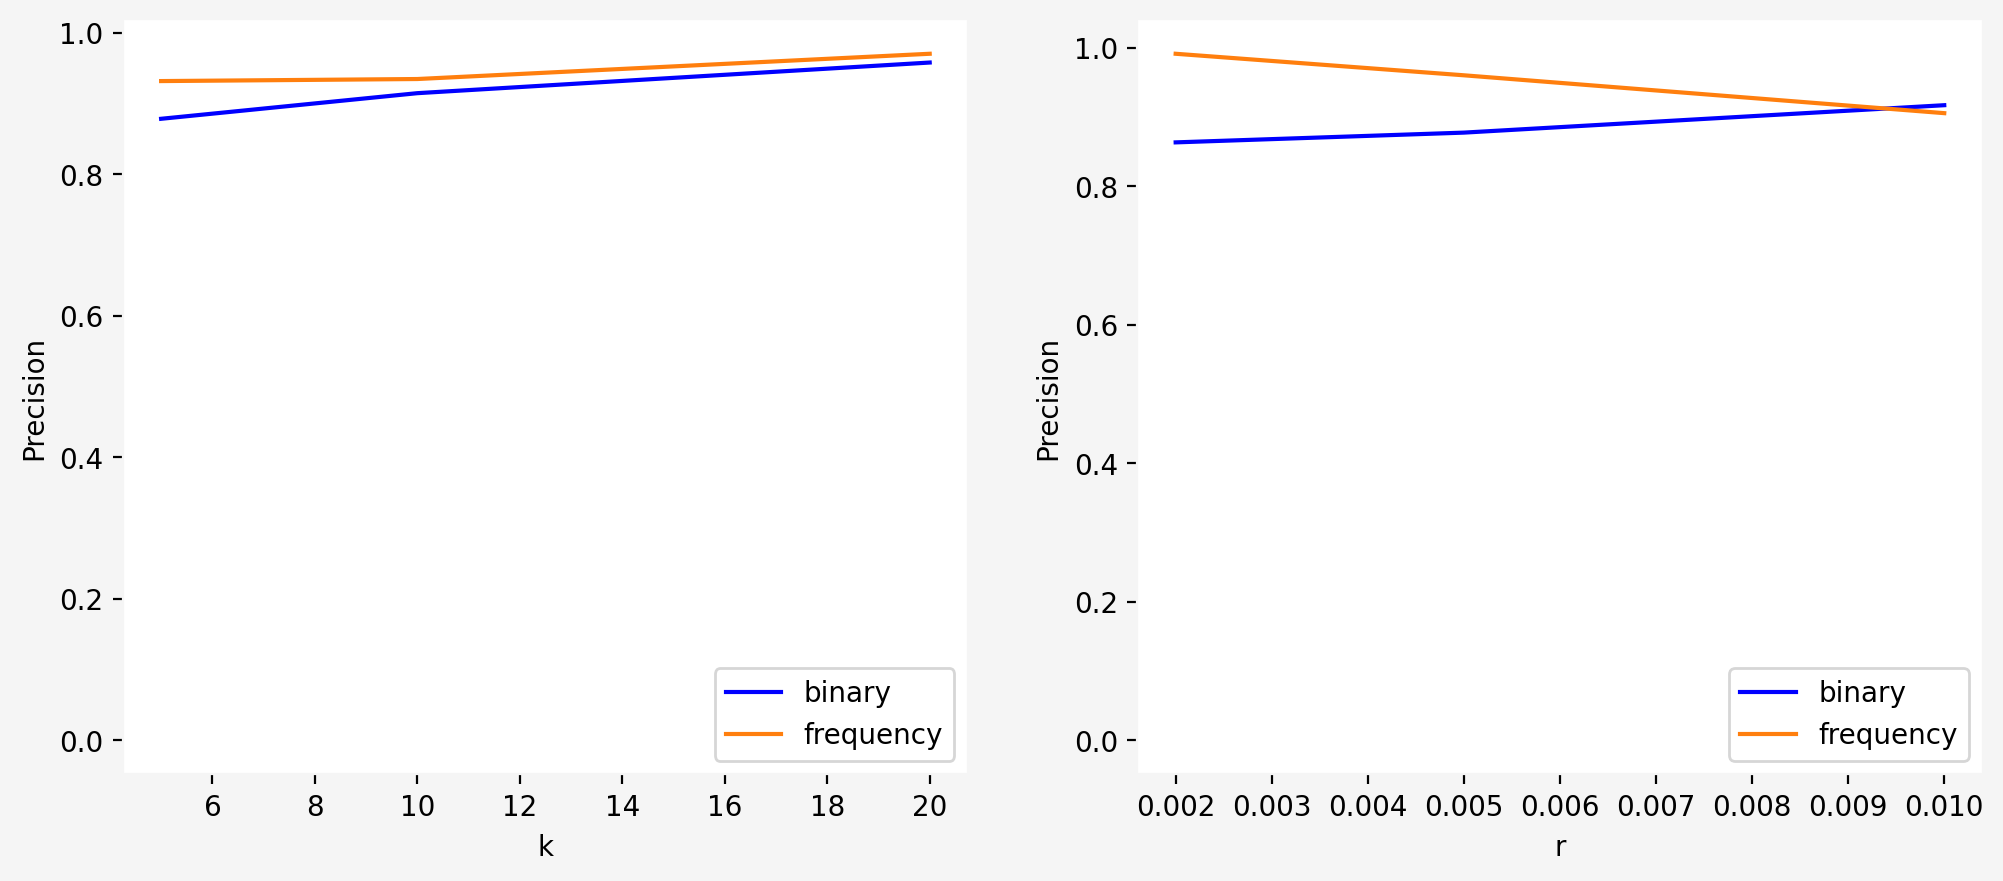
\includegraphics[width=1 \textwidth]{Precision} 
\end{figure}
\end{block}
\end{frame}


\begin{frame}
\frametitle{MAP} 
\begin{block}{} \vspace{-1cm}
\begin{figure}[h] 
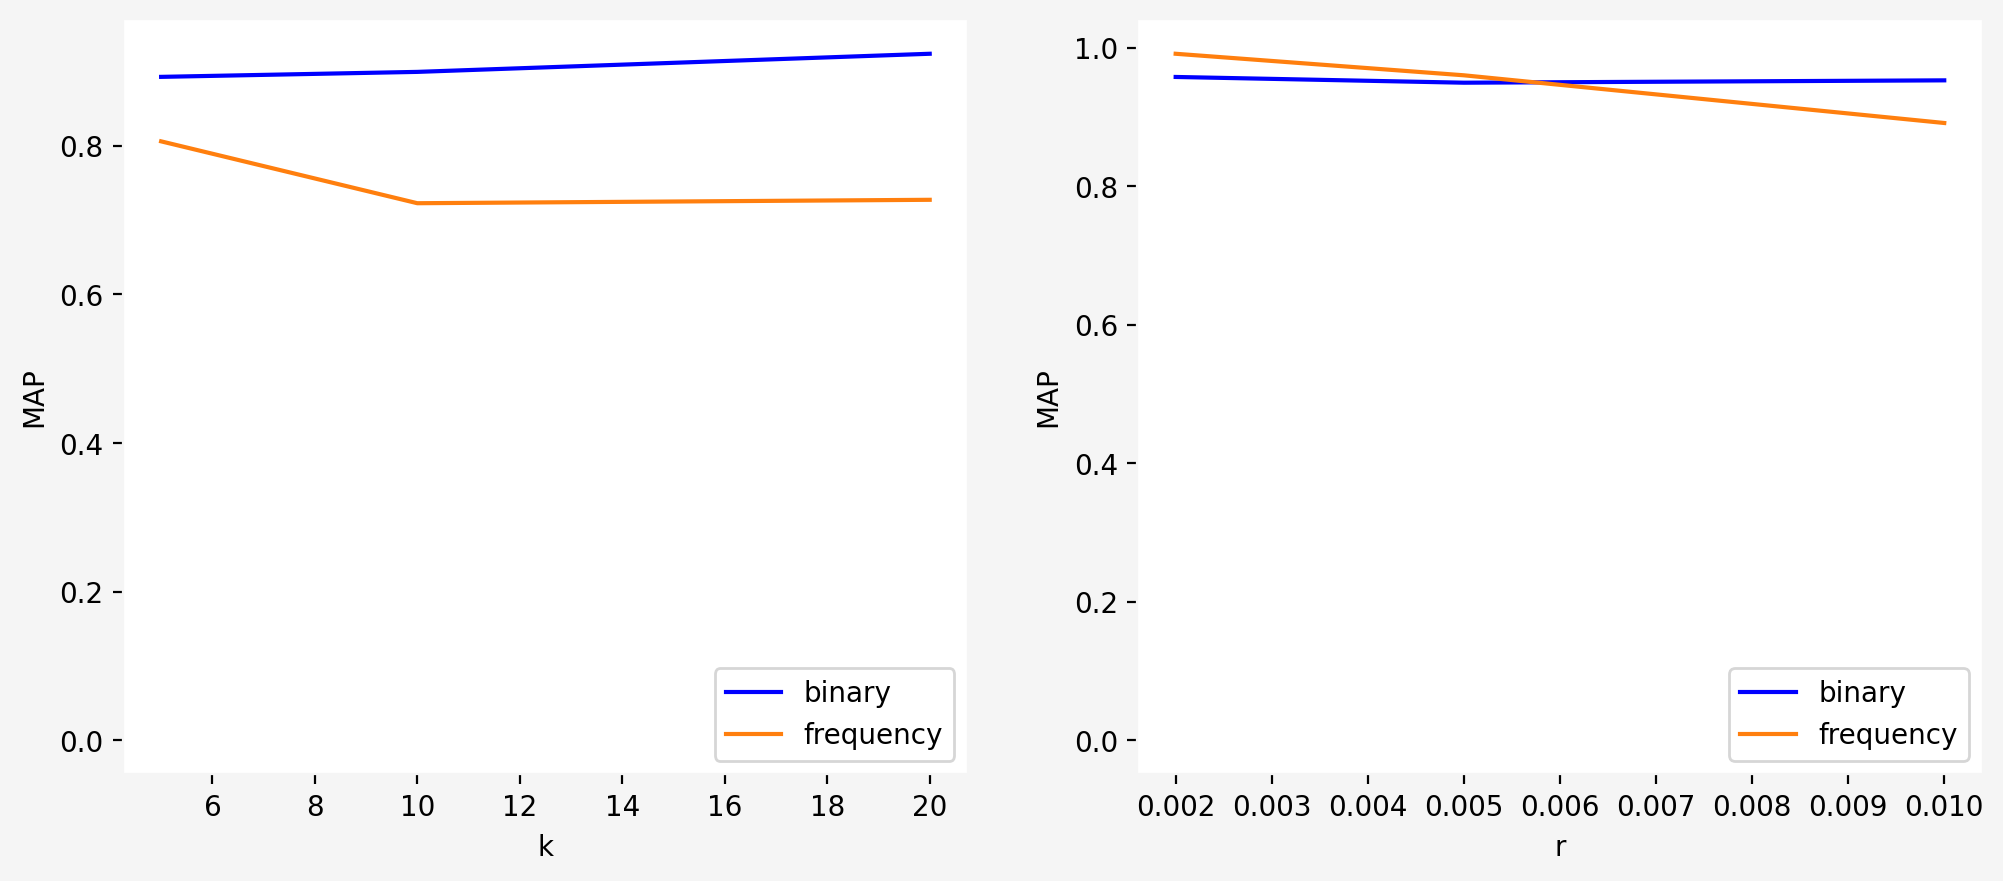
\includegraphics[width=1 \textwidth]{MAP}
\end{figure}
\end{block}
\end{frame}


\begin{frame}
\frametitle{nDCG} 
\begin{block}{} \vspace{-1cm}
\begin{figure}[h] 
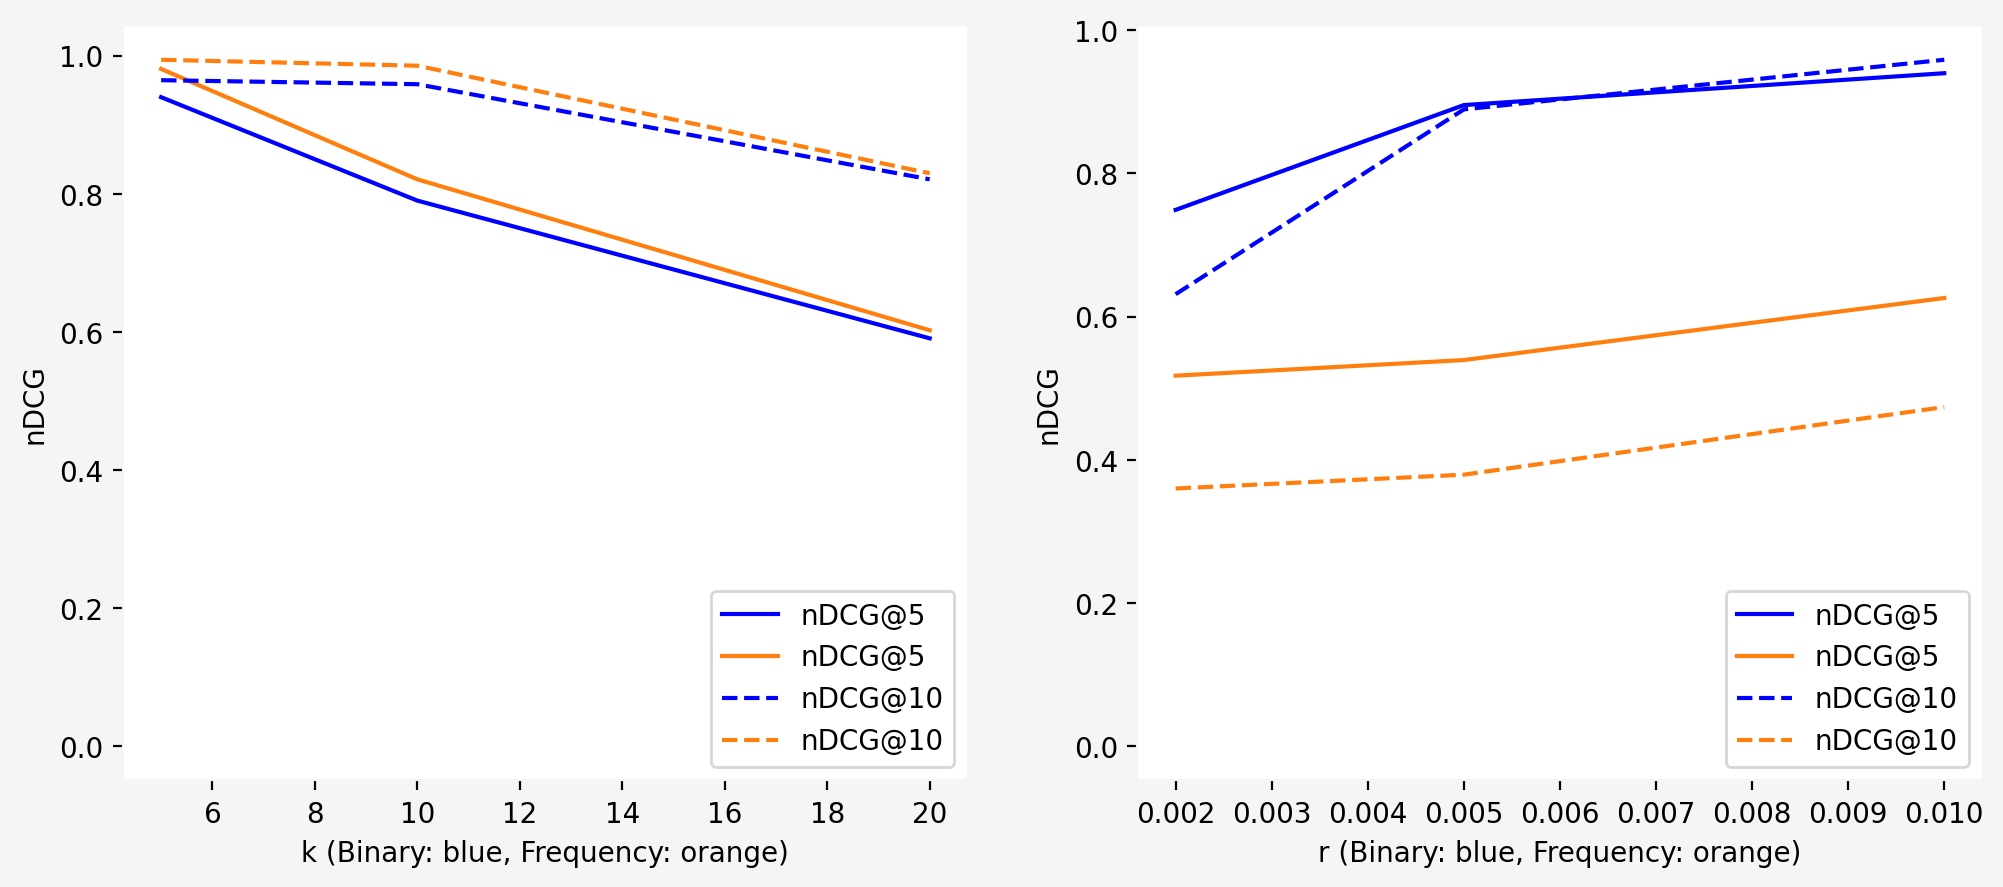
\includegraphics[width=1 \textwidth]{nDCG} 
\end{figure}
\end{block}
\end{frame}


\begin{frame}
\frametitle{kNN/Range Queries Using DTW (Car-Bus)} 
\begin{block}{} \vspace{-5mm}
\begin{table}[!htbp]
{\footnotesize
\centering
\begin{tabular}{rccccc}
 	{\bf k } 	& {\bf Precision/Recall}	&	{\bf MAP}	 & {\bf nDCG@5}	& {\bf nDCG@10} \\ \midrule
 	5   		& 	0.5600   		 	&	0.6580	 & 0.7391			& 0.8088	\\ \midrule
	10   		& 	0.5381    		 	&	0.6022	 & 0.5991			& 0.7170	\\ \midrule
 	20  		&   	0.5090   			&	0.5569	 & 0.4513  		& 0.5862	\\ \bottomrule 
\end{tabular}  \vspace{5mm}

\centering
\begin{tabular}{rccccc}
 	{\bf r } 	& {\bf Precision}& {\bf Recall}	&	{\bf MAP}	 & {\bf nDCG@5}	& {\bf nDCG@10} \\ \midrule
 	0.002   	& 	0.5752    	& 	0.9952	&	0.4961	 & 0.5957			& 0.4550	\\ \midrule
	0.005   	& 	0.3647    	& 	0.9514 	&	0.1624	 & 0.6543			& 0.5305	\\ \midrule
 	0.01 		&   	0.3705  	&      0.8763	&	0.0634	 & 0.6913  		& 0.5860	\\ \bottomrule
\end{tabular} 
\caption{\footnotesize Performance with DTW as ground truth distance (binary representation)}
\label{table: car-bus binary dtw} 
}
\end{table}
\end{block}
\end{frame}


%%%%%%%%%%%%%%%%%%% Geolife

\subsection{Geolife}

\begin{frame}
\frametitle{kNN Queries (Geolife)} 
\begin{block}{} \vspace{-3mm}
\begin{table}[!htbp]
{\footnotesize
\centering
\begin{tabular}{rcccc}
 	{\bf k } 	& {\bf Precision/Recall}	&	{\bf MAP}	 & {\bf nDCG@5}	& {\bf nDCG@10} \\ \midrule
 	 5   		& 	0.8676   			&	0.8632	& 0.9182		& 0.9443	\\ \midrule
	10   		& 	0.8921    		 	&	0.8751	& 0.7822		& 0.9394	\\ \midrule
 	20  		&   	0.9074   			&	0.8904	& 0.5823  		& 0.7989	\\ \bottomrule\end{tabular} 
\caption{\footnotesize Performance with binary representation} \vspace{3mm}

\centering
\begin{tabular}{rcccc}
 	{\bf k } 	& {\bf Precision/Recall}	&	{\bf MAP}	 & {\bf nDCG@5}	& {\bf nDCG@10} \\ \midrule
 	 5   		& 	0.9480   		 	&	0.9597	 & 0.9822			& 0.9930	\\ \midrule
	10   		& 	0.9590    		 	&	0.9577	 & 0.8233			& 0.9886	\\ \midrule
 	20  		&   	0.9653   			&	0.9604	 & 0.6029  		& 0.8330	\\ \bottomrule
\end{tabular} 
\caption{\footnotesize Performance with frequency representation}
\label{table: Geolife binary} 
}
\end{table}
\end{block}
\end{frame}



\begin{frame}
\frametitle{Range Queries (Geolife)} 
\begin{block}{} \vspace{-3mm}
\begin{table}[!htbp]
{\footnotesize
\centering
\begin{tabular}{rccccc}
 	{\bf r } 	& {\bf Precision}& {\bf Recall}	&	{\bf MAP}	 & {\bf nDCG@5}	& {\bf nDCG@10} \\ \midrule
  	0.001   	& 	0.9275    	& 	0.9549 	&	0.8116	& 0.7260		& 0.6559	\\ \midrule
	0.005   	& 	0.8896    	& 	0.9023 	&	0.2025	& 0.8893		& 0.8952	\\ \midrule
 	0.01	 	&   	0.8883   	&      0.8892	&	0.0376	& 0.9182  		& 0.9390	\\ \bottomrule
\end{tabular} 
\caption{\footnotesize Performance with binary representation} \vspace{3mm}

\centering
\begin{tabular}{rccccc}
 	{\bf r } 	& {\bf Precision}& {\bf Recall}	&	{\bf MAP}	 & {\bf nDCG@5}	& {\bf nDCG@10} \\ \midrule
  	0.001   	& 	0.9990    	& 	1		&	0.9990	 & 0.4906			& 0.3367	\\ \midrule
	0.005   	& 	0.9894    	& 	1		&	0.9973	 & 0.5291			& 0.3748	\\ \midrule
 	0.01	 	&   	0.9765   	&      0.9978	&	0.9582	 & 0.5735  			& 0.4276	\\ \bottomrule
\end{tabular} 
\caption{\footnotesize Performance with frequency representation}
\label{table: Geolife multipass} 
}
\end{table}
\end{block}
\end{frame}



\begin{frame}
\frametitle{Precision} 
\begin{block}{} \vspace{-1cm}
\begin{figure}[h] 
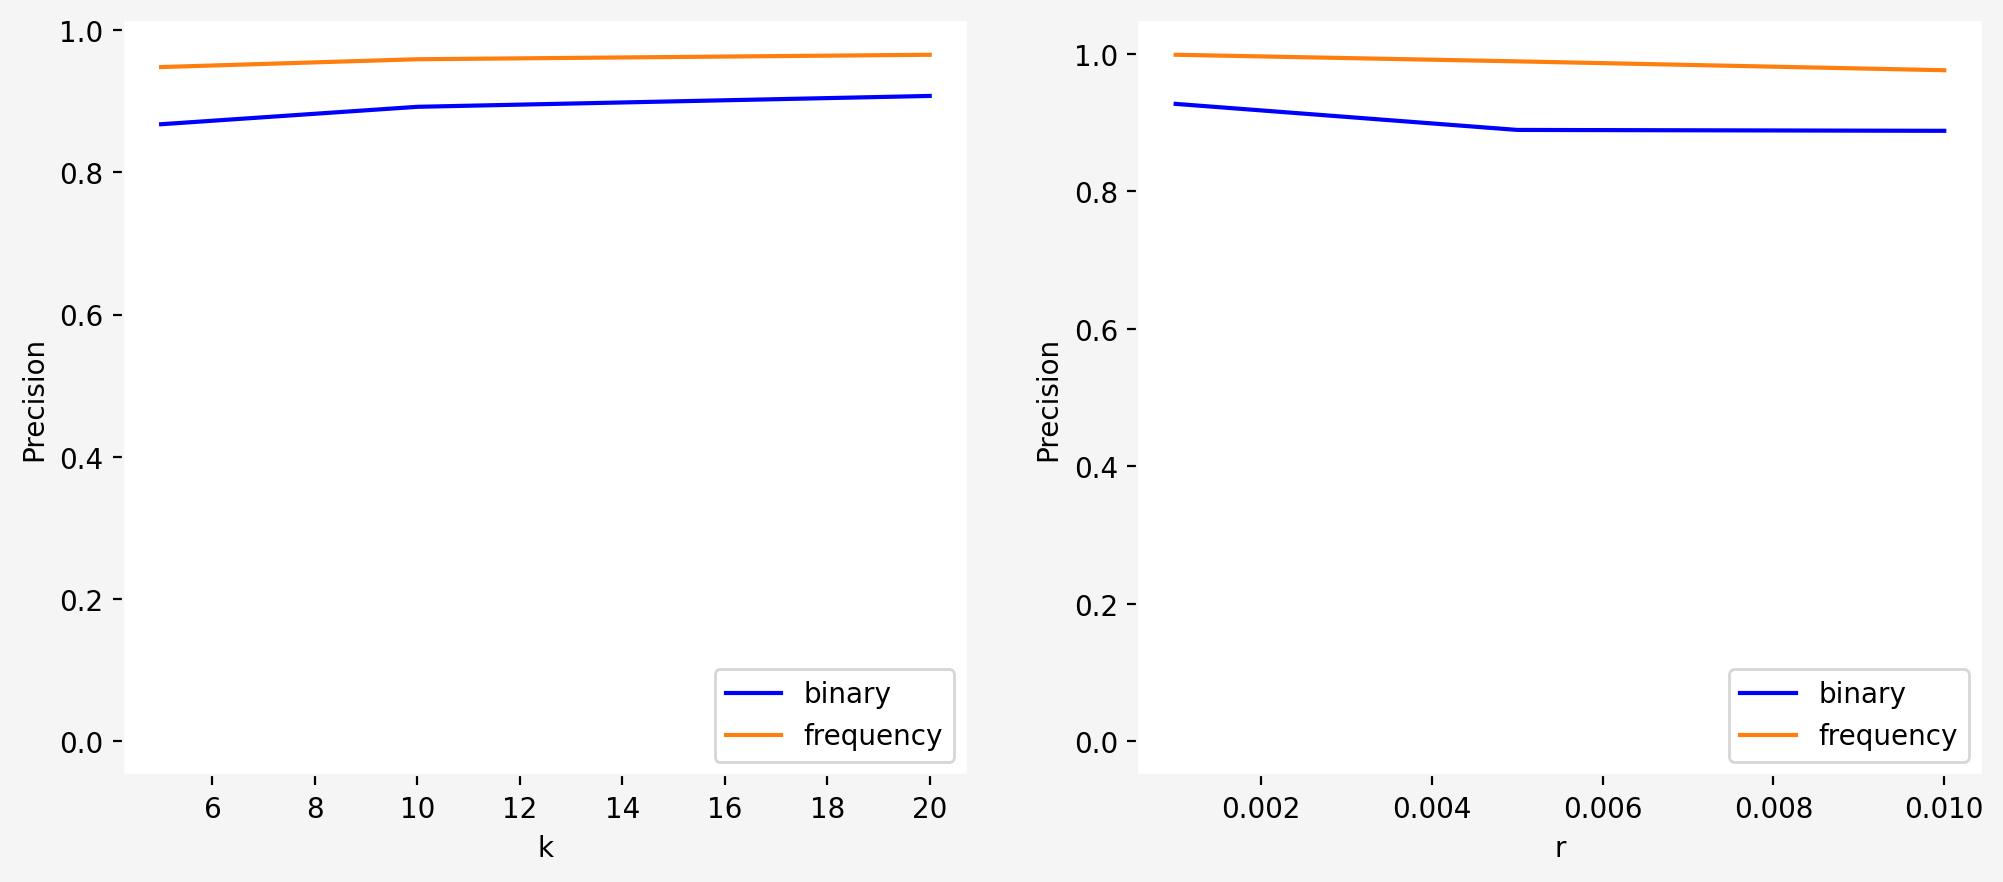
\includegraphics[width=1 \textwidth]{Precision-Geolife} 
\end{figure}
\end{block}
\end{frame}


\begin{frame}
\frametitle{MAP} 
\begin{block}{} \vspace{-1cm}
\begin{figure}[h] 
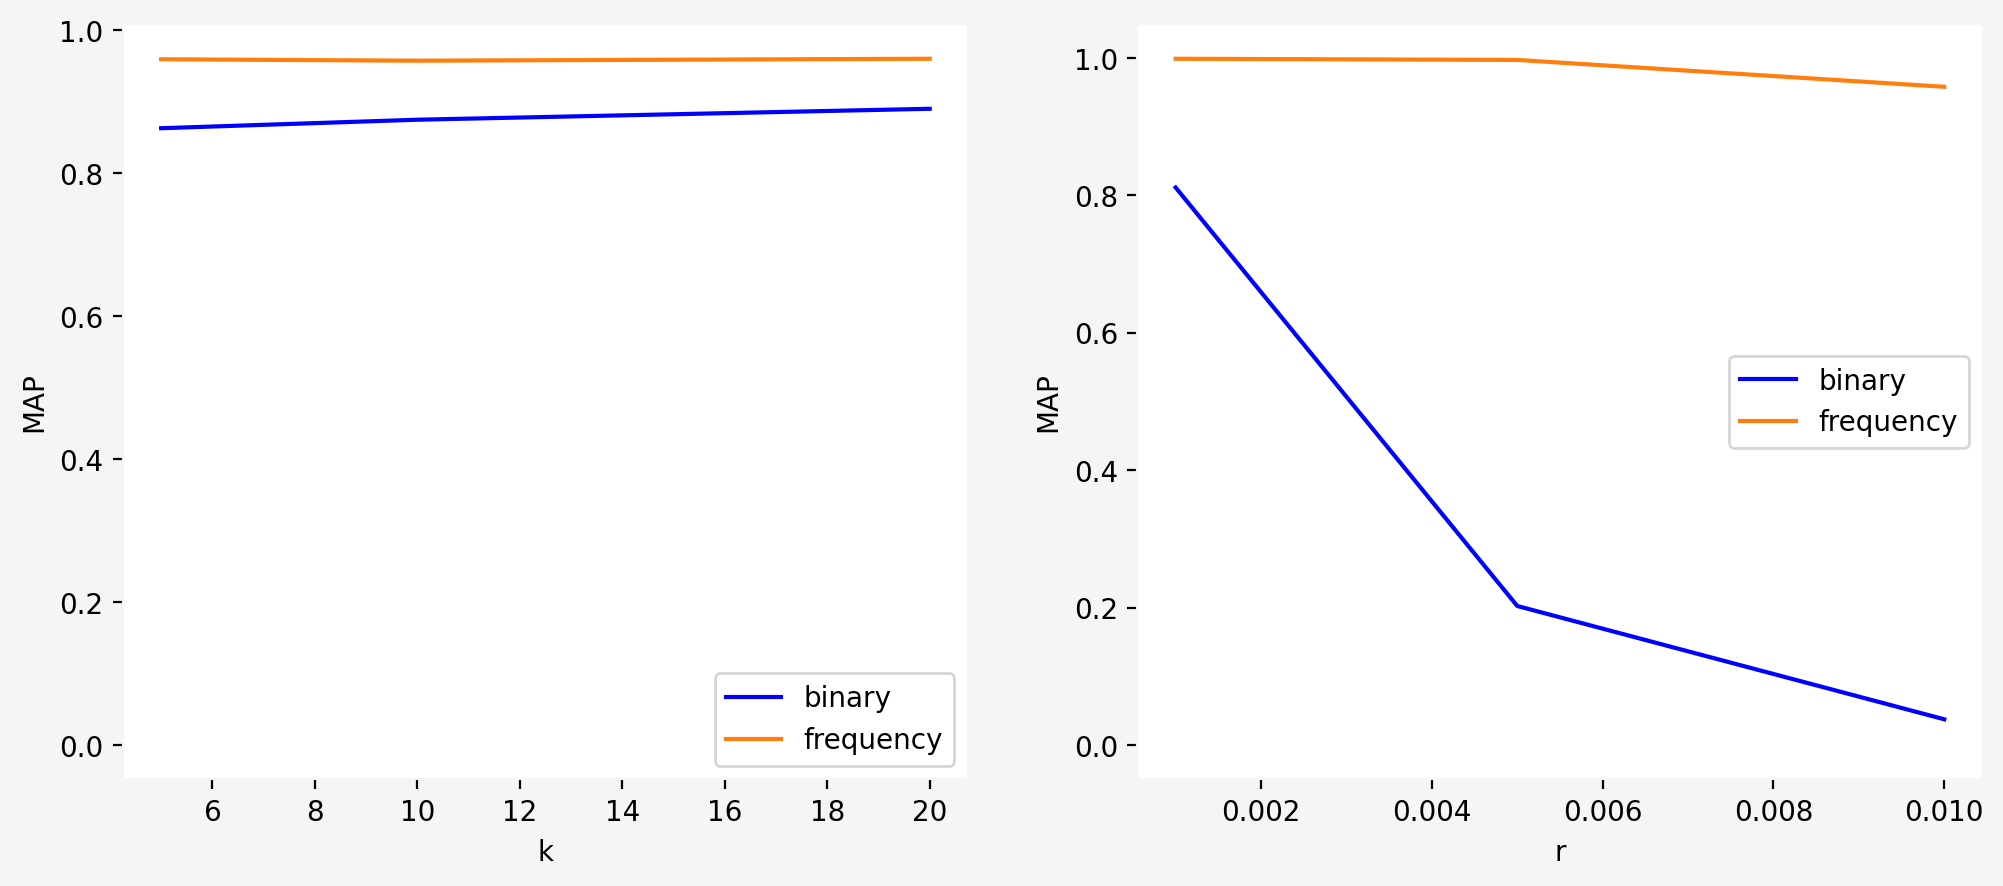
\includegraphics[width=1 \textwidth]{MAP-Geolife}
\end{figure}
\end{block}
\end{frame}


\begin{frame}
\frametitle{nDCG} 
\begin{block}{} \vspace{-1cm}
\begin{figure}[h] 
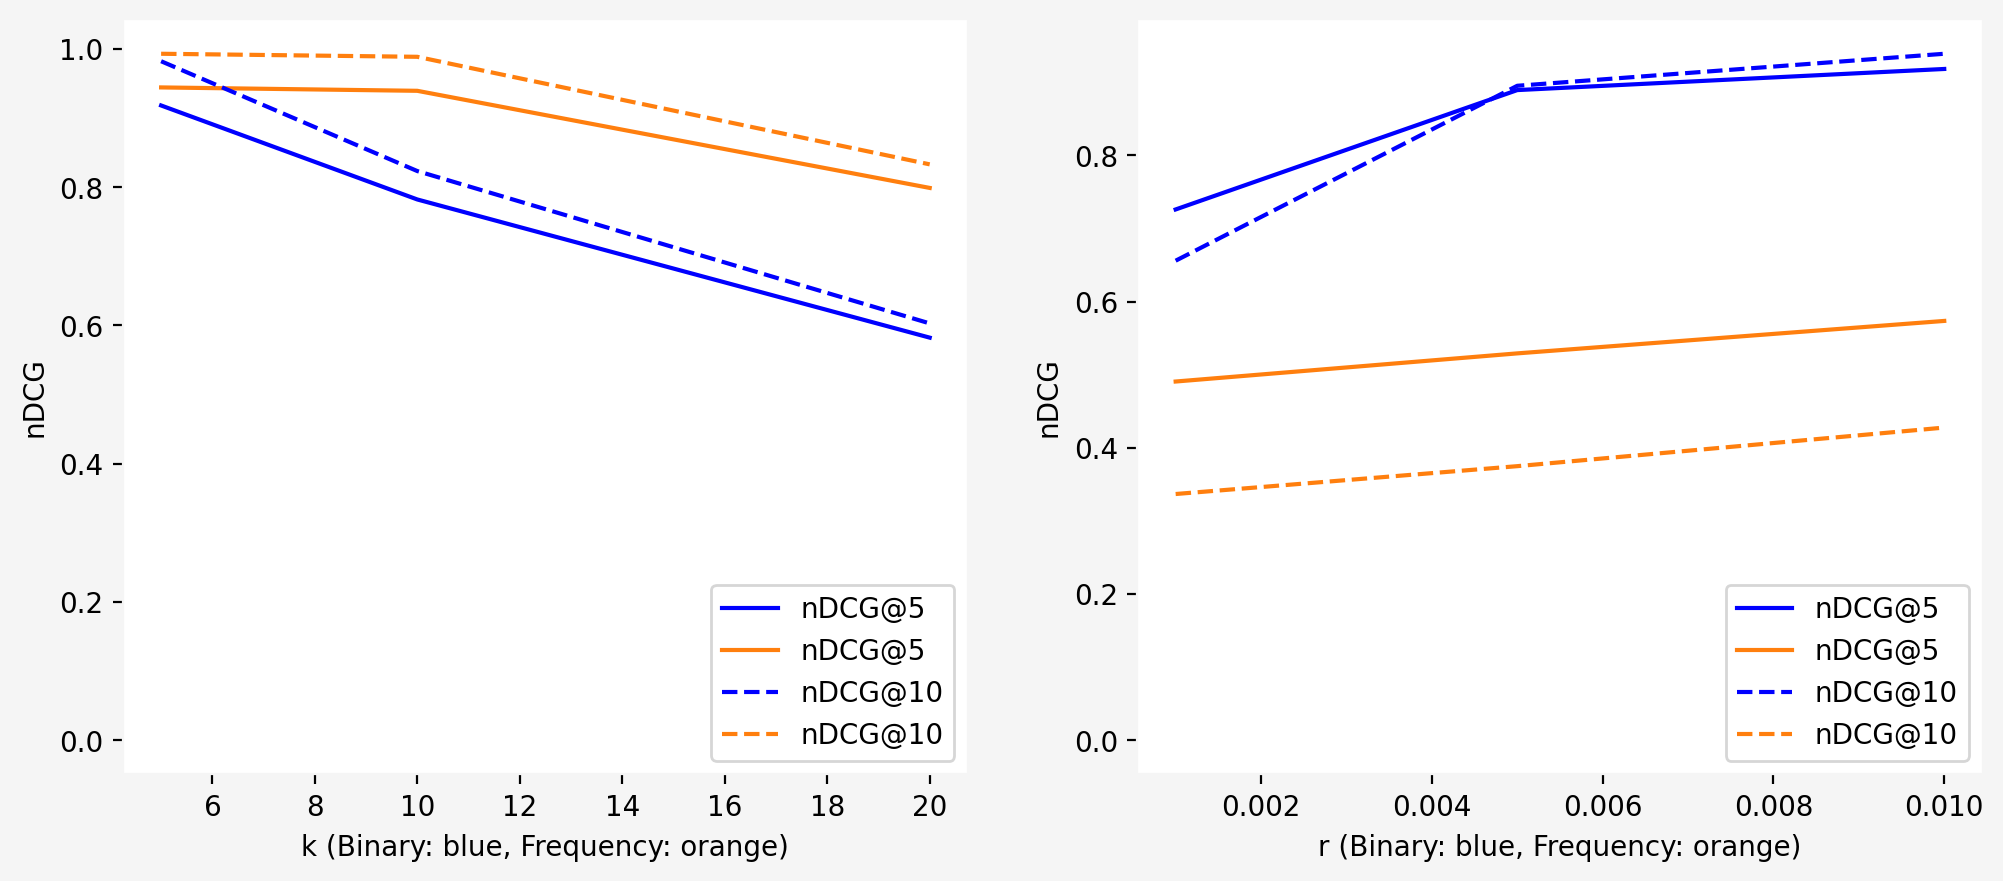
\includegraphics[width=1 \textwidth]{nDCG-Geolife} 
\end{figure}
\end{block}
\end{frame}


%%%%%%%%%%%%%%%%%%%%%%%%%%%%


\section{Conclusion}

\begin{frame}
\frametitle{Conclusion} 
\begin{block}{}
\begin{itemize}
\item LSI technique for trajectory retrieval is a quite successful one, \pause
\item The frequency-type representation tended to perform better in terms of AP, Recall and MAP, \pause
\item The binary representation tended to perform better in terms of nDCG, \pause
\item LSI technique works better with GAD in comparison to DTW distance, \pause
\item Increasing the number of grids leads to a better performance, \pause
\item Increasing the number of dimensions in dimensionality reduction technique leads to a better performance.
\end{itemize}
\end{block}
\end{frame}



%%%%%%%%%%%%%%%%%%%%%%%%%%%%


\section{Contributions}

\begin{frame}
\frametitle{My Contributions} 
\begin{block}{}
\begin{itemize}
\item Applying a kernel-based similarity measure,
\item Using 3 different datasets as benchmark including a big data, 
\item Utlizing binary vectorization of trajectories,
\item Using term-frequency type trajectory vectorization, 
\item Applying DTW as a ground truth distance, 
\item Creating a user-friendly interactive search tool for kNN and range queries of trajectories. 
\end{itemize}

\end{block}
\end{frame}




\section*{Questions/Comments}
{\color{white}1}
\begin{center} 
{\huge \color{magenta}{\sc \vspace{3cm} Questions?}}
\end{center}


































\end{document}